% !TeX root = ../main.tex

\chapter{系统测试和分析}

软件测试是软件开发的最后一道程序,分为功能性测试和非功能性
测试。功能性测试是为了保证需求分析中的预期功都能实现,给用户提供满意的
服务。非功能性测试是为了保证软件的性能及可持续发展,主要侧重于
系统的可维护性、扩展性、健壮性和兼容性等。此外,对于安全性要求较高的软件
系统,还需要进行大量的安全性测试以保证系统的安全性。本章将对上一章实现的中文时间表达式信息抽取系统进行测试,其主
要目的是验证本中文时间表达式信息抽取系统能否准确有效地支持中文时间表达式的识别解析,解析结果能否正确地存储到数据库中,以及是否完成用户界面的设计和渲染。

\section{测试方案}

系统采用单元测试的方式对各个模块的功能函数进行正确性测试,在提供的测试环境中对系统的各项功能进行功能性测试,对系统整体的性能做性能测试,
最后对测试结果进行详细的分析和总结。主要的测试方案如下:

\begin{enumerate}
    \item[(1)] Web客户端:通过浏览器访问本系统,在web页面上的组件上发送各类查询需求,检查返回数据是否完整,页面渲染是否符合预期结果;
    \item[(2)] 服务端:对 web 客户端的查询请求进行解析和检查,检查查询请求是否能正确到达服务端,并且被服务端处理。根据服务端的资源消耗分析系统的性能瓶颈;
    \item[(3)] 数据库:通过对数据库接口进行测试,检查数据库接口对于指定的查询是否能返回正确数据,数据库对查询请求的响应时间是否达到要求;
    \item[(4)] 对客户端、服务端以及数据库访问接口模块中的代码做单元测试。
\end{enumerate}

\begin{table}[h]
    \centering
    \caption{服务测试环境}
    \begin{tabular}{|*{3}{c|}}
        \hline
        项目       & 软件               & 版本   \\
        \hline
        操作系统   & CentOS             & 7      \\
        \hline
        编辑器     & Visual Studio Code & 1.41   \\
        编程语言   & Python             & 3.7.2  \\
        \hline
        代理服务器 & Nginx              & 1.17.2 \\
        \hline
        工具库     & SciKit-learn       & 0.21.1 \\
        \hline
        内存       & 8G                 &        \\
        \hline
        CPU        & Intel              & 7900K  \\
        \hline
    \end{tabular}
    \label{tab:server_test}
\end{table}

\begin{table}[b]
    \centering
    \caption{单元测试方案表}
    \newcolumntype{Y}{>{\centering\arraybackslash}X}
    \begin{tabularx}{\linewidth}{|Y|Y|Y|Y|}
        \hline
        测试项                                     & 测试步骤                                                                                                         & 预期结果                           & 实际结果                           \\
        \hline
        中文时间表达式信息抽取模块配置加载失败     & 构造中文时间表达式信息抽取模块配置文件参数使得某些重要参数缺失,随后启动中文时间表达式信息抽取模块。             & 中文时间表达式信息抽取模块启动失败 & 中文时间表达式信息抽取模块启动失败 \\
        \hline
        中文时间表达式信息抽取模块配置加载异常     & 构造中文时间表达式信息抽取模块配置文件参数,在配置文件中设置错误的参数类型,随后启动中文时间表达式信息抽取模块。 & 中文时间表达式信息抽取模块启动失败 & 中文时间表达式信息抽取模块启动失败 \\
        \hline
        中文时间表达式信息抽取模块配置加载成功     & 构造中文时间表达式信息抽取模块配置文件参数,给予配置文件中正确的配置参数启动中文时间表达式信息抽取模块。         & 中文时间表达式信息抽取模块启动成功 & 中文时间表达式信息抽取模块启动成功 \\
        \hline
        中文时间表达式信息抽取模块文本信息抽取失败 & 构造错误的文本并调用解析接口,再调用信息抽取模块算法解析上传文本。                                               & 中文时间表达式信息抽取模块抽取失败 & 中文时间表达式信息抽取模块抽取失败 \\
        \hline
        中文时间表达式信息抽取模块文本信息抽取成功 & 构造正确的文本并调用解析接口,再调用信息抽取模块算法解析上传文本。                                               & 中文时间表达式信息抽取模块抽取成功 & 中文时间表达式信息抽取模块抽取成功 \\
        \hline
    \end{tabularx}
    \label{tab:unit_test1}
\end{table}


\begin{table}[h]
    \centering
    \renewcommand\thetable{6.2}
    \caption{(续)单元测试方案表}
    \newcolumntype{Y}{>{\centering\arraybackslash}X}
    \begin{tabularx}{\linewidth}{|Y|Y|Y|Y|}
        \hline
        测试项                  & 测试步骤                                                     & 预期结果                                                   & 实际结果                                                     \\
        \hline
        MongoDB插入失败         & 构造错误的数据类型并调用数据存取模块接口插入错误的数据类型。 & 数据库插入失败,日志系统报错                               & 数据库插入失败,日志系统报错                                 \\
        \hline
        MongoDB插入成功         & 构造正确的数据类型并调用数据存取模块接口插入正确的数据类型。 & 数据库插入成功,日志系统正常打印日志,接口返回成功消息     & 数据库插入成功,日志系统正常打印日志,接口返回成功消息       \\
        \hline
        MongoDB查询不存在的数据 & 根据MongoDB集合中已有的唯一索引构造不存在的索引进行查询。    & 数据库返回为空,日志系统正常打印日志,接口返回成功消息     & 数据库返回为空,日志系统正常打印日志,接口返回成功消息       \\
        \hline
        MongoDB查询存在的数据   & 根据MongoDB集合中已有的唯一索引随机选取多条查询。            & 数据库返回正确数据,日志系统正常打印日志,接口返回成功消息 & 数据库返回正确数据, 日志系统正常打印日志, 接口返回成功消息 \\
        \hline
        数据库连接失败          & 给定错误的数据库连接参数并调用数据库连接接口。               & 数据库连接失败                                             & 数据库连接失败                                               \\
        \hline
    \end{tabularx}
    \label{tab:unit_test2}
\end{table}


\section{测试环境}

本中文时间信息抽取可以部署在 Linux 和 Windows 系统环境中。在实际的应用中,Linux相较Windows更为稳定,且服务部署方案也更成熟,故将系统部署到Linux的发行版Ubuntu上。

服务端测试环境部署实例为4台实例,其中三台为服务处理实例,一台为MongoDB实例。服务实例环境见表~\ref{tab:server_test}。



\section{单元测试}

\subsection{单元测试概述}

单元测试主要对本地部署的服务端实例的正确性进行测试,本系统采用Python语言的pytest单元测试框架进行测试,通过命令行运行pytest测试指令,检查测试结果的正确性。

\subsection{单元测试方案设计}

% TODO: 修改
本地部署的服务端实例的单元测试采用 Python 语言的 pytest 单元测试框架,服务端单元测
试方法主要针对本系统的中文时间表达式信息识别模块、解析模块以及数据库持久化存储的接口,对模块中出现的所有功能函数可能出现的错误或者异常结果进行测试和路径覆盖,
主要的测试用例如下表~\ref{tab:unit_test1}所示。

\section{功能性测试}

\begin{table}[hbt]
    \centering
    \renewcommand\thetable{6.3}
    \caption{功能测试方案表}
    \newcolumntype{Y}{>{\centering\arraybackslash}X}
    \begin{tabularx}{\linewidth}{|Y|Y|Y|}
        \hline
        测试项                           & 预期结果                                                 & 实际结果                                                 \\
        \hline
        每日表达式识别失败数量           & 成功获取到每日表达式识别失败数量,并返回给前端           & 成功获取到每日表达式识别失败数量,并返回给前端           \\
        \hline
        每日表达式解析失败数量           & 成功获取到每日表达式解析失败数量,并返回给前端           & 成功获取到每日表达式解析失败数量,并返回给前端           \\
        \hline
        每日表达式识别与解析用户调用数量 & 成功获取到每日表达式识别与解析用户调用数量,并返回给前端 & 成功获取到每日表达式识别与解析用户调用数量,并返回给前端 \\
        \hline
        每日 OCR 模块调用数量            & 成功获取到每日 OCR 模块调用数量,并返回给前端            & 成功获取到每日 OCR 模块调用数量,并返回给前端            \\
        \hline
        每日表达式识别失败分析           & 成功获取到每日表达式识别失败数量,并返回给前端           & 少部分样例识别失败无分析,可获取失败分析可成功返回前端   \\
        \hline
        每日表达式解析失败分析           & 成功获取到每日表达式解析失败分析,并返回给前端           & 成功获取到每日表达式解析失败分析,并返回给前端           \\
        \hline
        单语句可视化分析                 & 成功获取到单语句可视化分析,并返回给前端                 & 成功获取到单语句可视化分析,并返回给前端                 \\
        \hline
    \end{tabularx}
    \label{tab:functional_test}
\end{table}

% TODO: 修改
功能测试主要对系统所有功能的完整性以及正确性进行测试,查看系统功
能是否满足预期功能需求,每项功能的运行结果是否正确。本节将主要对
系统数据分析和展示模块进行功能测试,确保Metis
页面能够查询到正确数据。在测试前,先将提前标注好的语料和相应的正确结果按多日多量的方式持续存入MongoDB中。
主要的测试用例如表~\ref{tab:functional_test} 所示。

同时将若干测试数据输入对应的UI测试页面,可以得到相应的结果,其结果如图~\ref{fig:web_result}所示。其中OPERATORROOT即为上文中提到的操纵符作为根节点识别到的结果,TIMEROOT则是文本作为准确的时间刻度识别到的文本。


\begin{figure}[h]
    \centering
    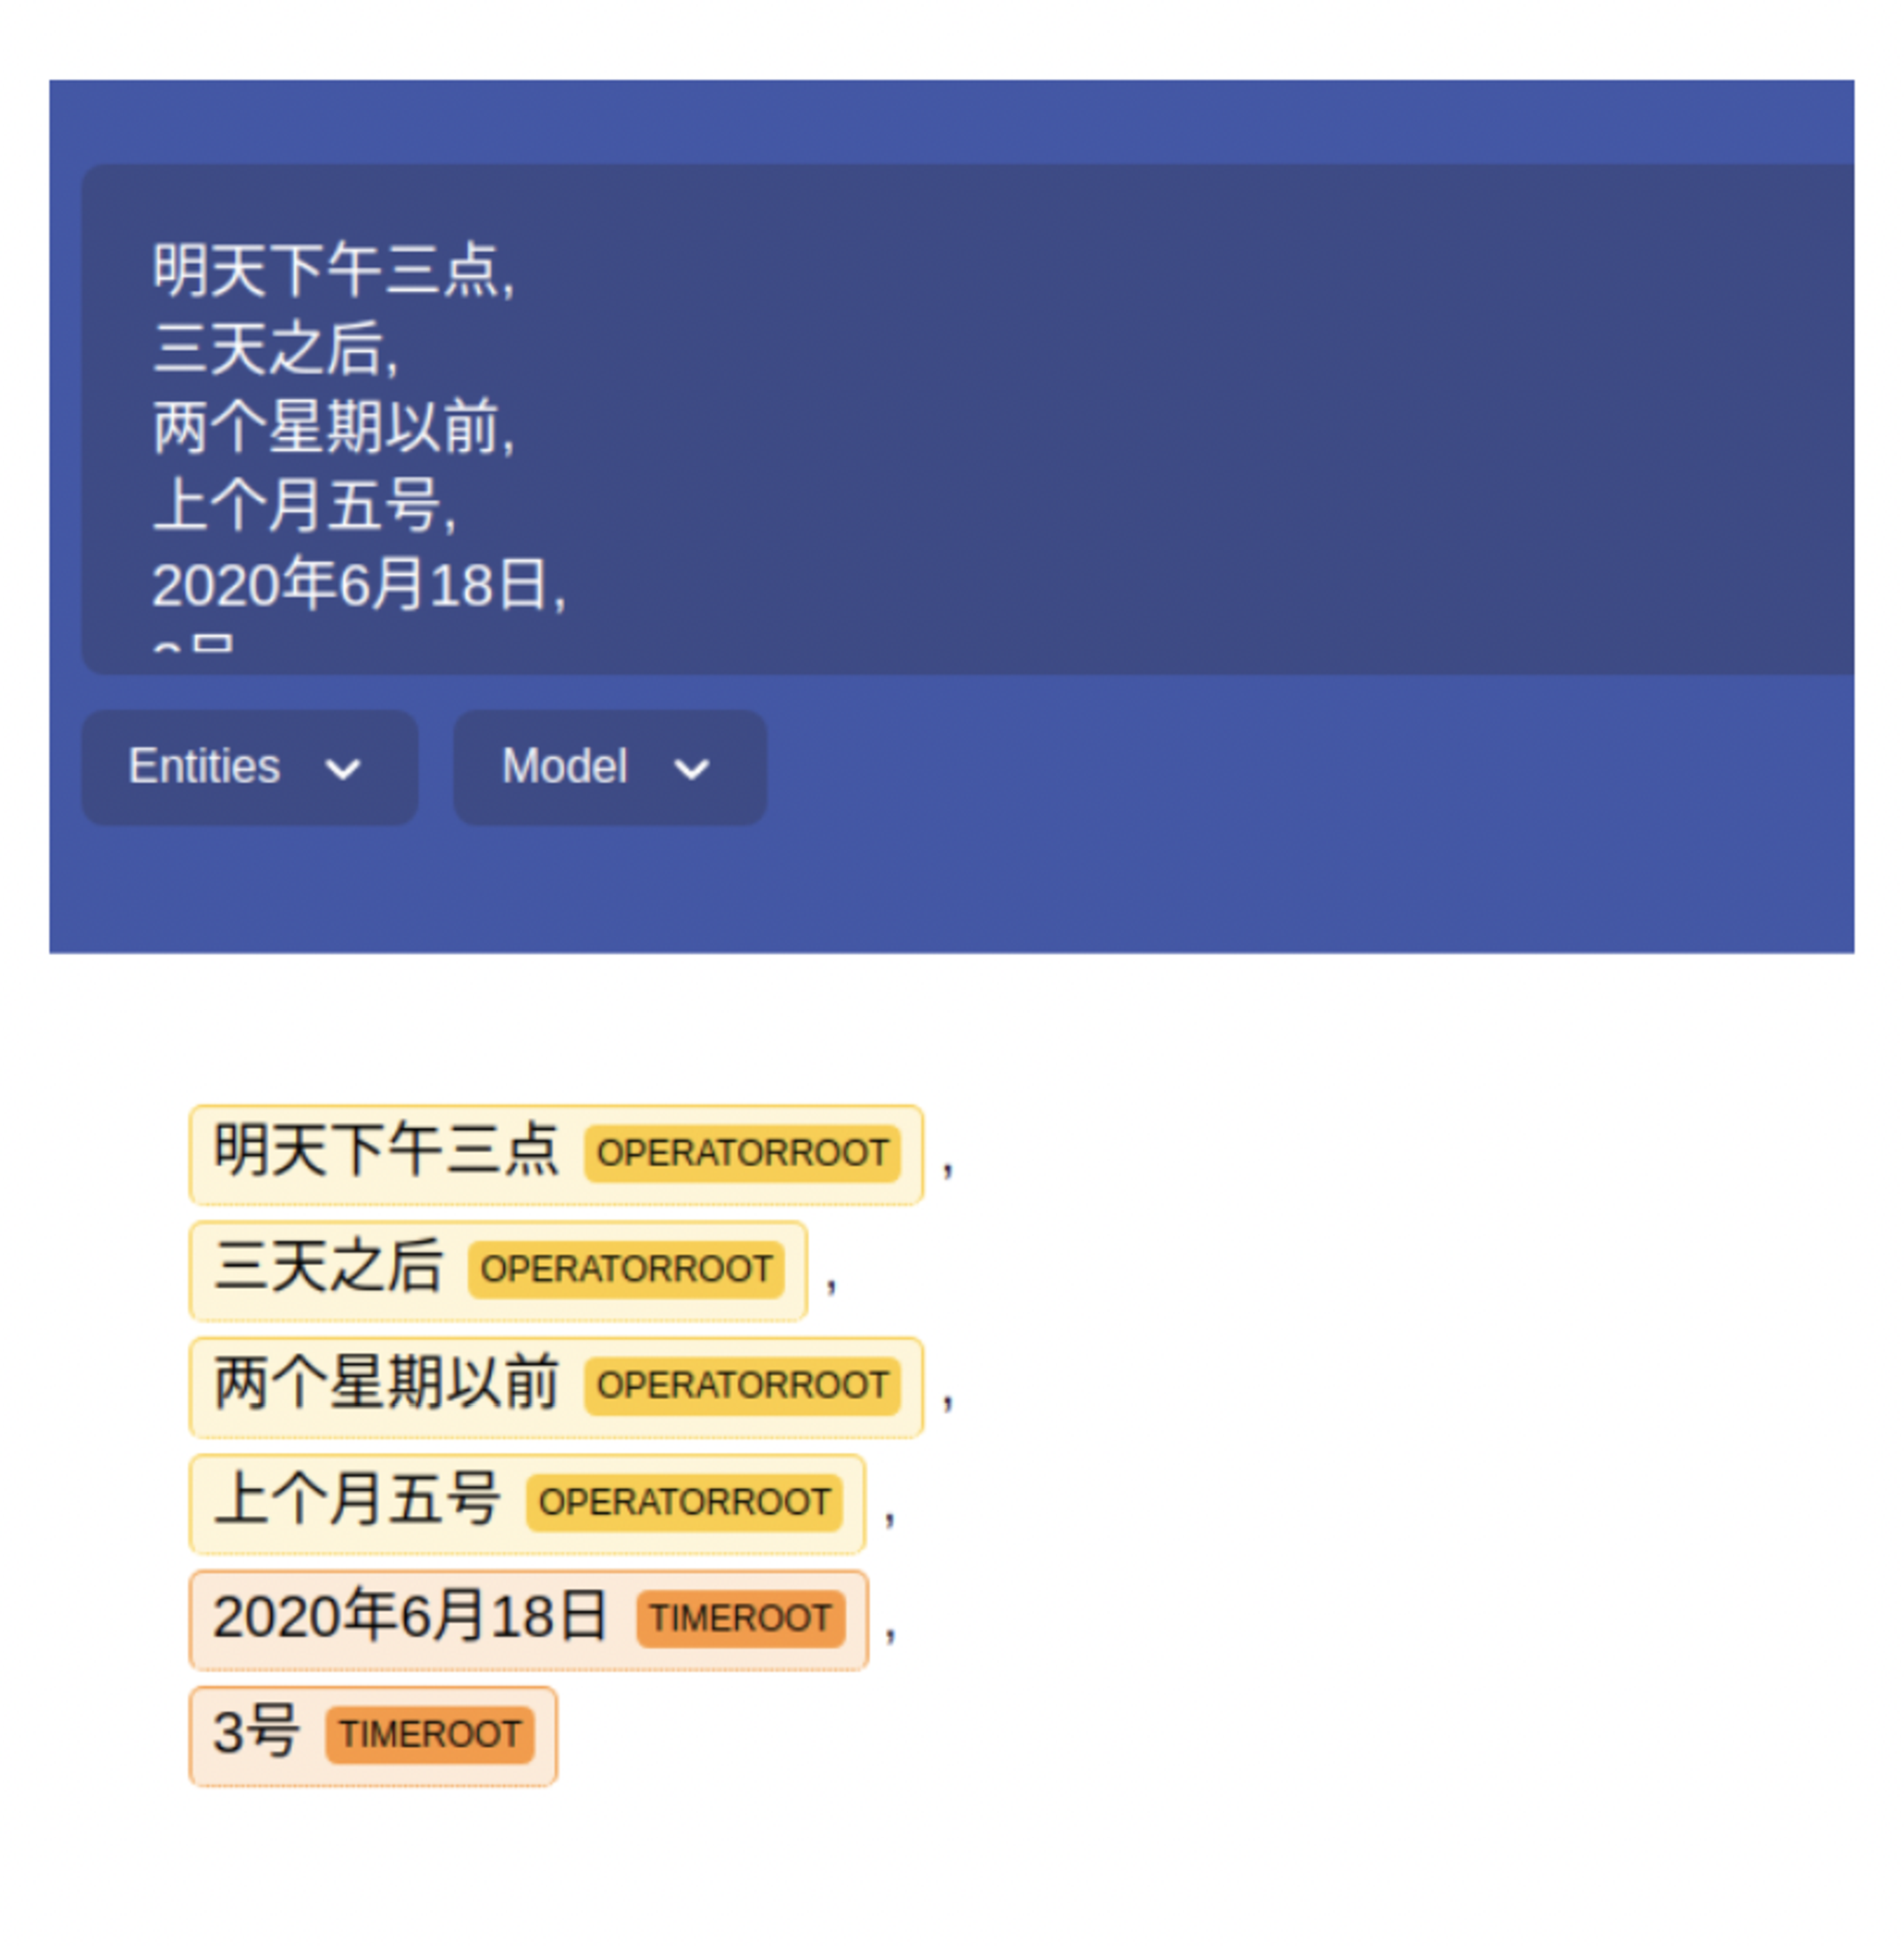
\includegraphics[width=0.7\textwidth]{web_result.pdf}
    \caption{UI测试页面}
    \label{fig:web_result}
\end{figure}

\section{非功能性测试}

\subsection{响应度和可用性测试}

\begin{figure}[t]
    \centering
    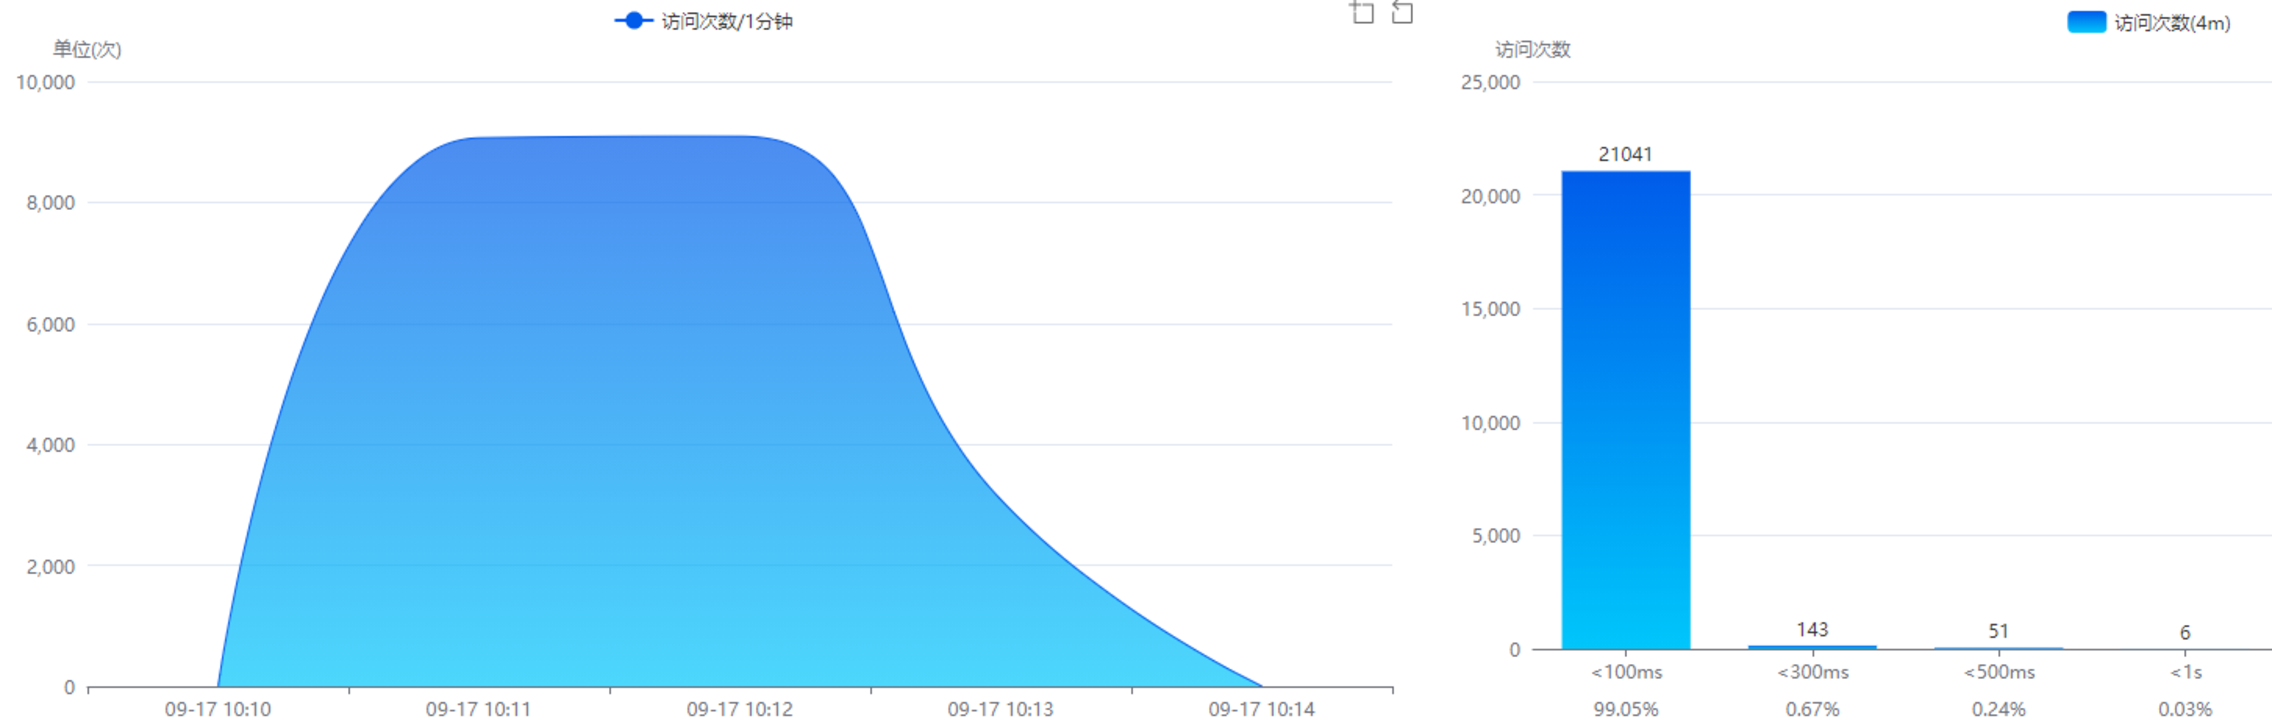
\includegraphics[width=1\textwidth]{pressure.pdf}
    \caption{压力测试图}
    \label{fig:pressure}
\end{figure}

为了满足响应度和可用性测试,采用Java的多线程压测工具Jmeter对服务器进行接口访问压测。逐步提高压测的线程数量和请求速度,
最终在日志系统中可以得到如图~\ref{fig:pressure}测试结果。由图可知百分之九十九的相应时间都落在一百毫秒以内,在每秒两百条请求时系统应用仍能持续运转。


\subsection{易用性测试}

本系统在提供给用户使用时,用户不需要关心数据库以
及前端页面的具体实现,只需根据自己的数据分析需求上传特定格式的文档即可,前端页面会自动渲染数据查询结果,以可视化的形式呈现数据查询结果。因此发布的中文时间表达式信息抽取系统满足易用性的需求。

\subsection{兼容性测试}

为了满足兼容性测试,本系统的前端 Metis 页面分别在谷歌浏览器、Edge
浏览器、火狐浏览器、360 浏览器进行了测试,以上浏览器均能在 Metis 页面
上呈现功能测试中的各项数据,因此本信息抽取系统对以上各种浏览器均能兼容。

\subsection{可维护性测试}

软件系统的可维护性可以用模块之间的耦合度、单元测试和集成测试的覆盖
率、代码规范性等指标进行度量。本系统在开发过程中采用面向对象的设计方法,严格
遵循单一责任、低耦合高内聚等原则来进行系统模块的设计,减少模块与模块之
间的耦合度、增加模块内部的功能复用。系统在开发过程中也会在关键代码处添
加日志,当异常和错误情况发生时,开发人员能够快速通过日志进行问题解决。
综合以上分析中文时间表达式信息抽取系统满足可维护性需求。


\section{本章小结}

本章主要介绍了中文时间表达式信息抽取系统的测试和验证过程,从单元测试、功能测试、非功能测试等方面对系统的功能完备性以及非功能需求做了相应的验证,
在单元测试和功能测试中列举了较为重要的测试用例,并详细说明了测试用例的测试过程和测试结果。
测试结果表明,本中文时间表达式信息抽取系统在准确性和实时性上都达到了预期,其他的非功能性需求也基本满足。
综上所述,本中文时间表达式信息抽取系统通过了有效测试,满足服务对象的需求。